\documentclass[12pt,oneside]{sotsuken_paper}

% タイトル
\title{ジャイロセンサを用いたロボットの方向自動修正}
\author{平元隆顕・松村隆平}

\begin{document}
% 行間
\setlength{\baselineskip}{9truemm}

%文字間
\kanjiskip=.53zw plus 3pt minus 3pt
\xkanjiskip=.53zw plus 3pt minus 3pt

% 目次
\tableofcontents
%\newpage

% 本文

\chapter{はじめに}

	\section{研究の背景}

		\subsection{2016年度「ロボット・ニューフロンティア」ルール説明}
		2016年度に行われたNHK高専ロボコンは「ロボット・ニューフロンティア」という題目で港町から海を渡り、新大陸へと目指すというものである。
		使用ロボット台数は無制限、港町で灯台を組み上げ、地に接触しないよう海を渡り、丘の上に砦を築く競技で今年は高さを競い合うものであった。図\ref{競技フィールド}はこの競技のフィールドである。


		\begin{figure}[htp]
			\begin{center}
				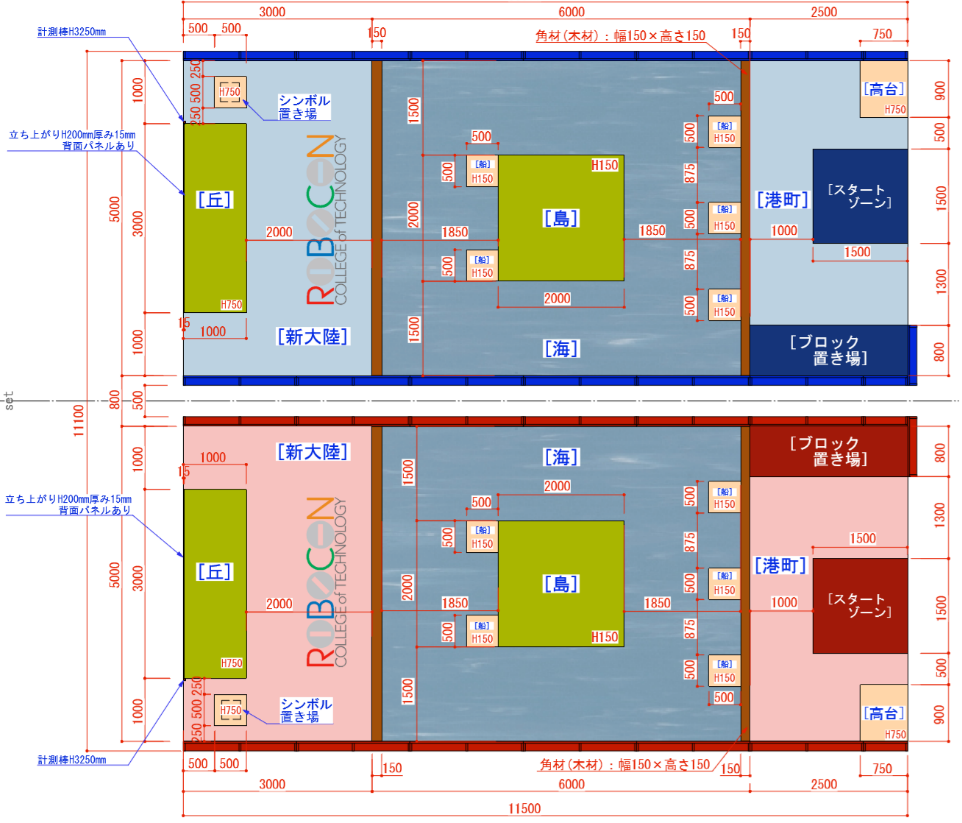
\includegraphics[width=80mm]{Image/フィールド.png}
				\caption{競技フィールド}
				\label{競技フィールド}
			\end{center}
		\end{figure}

	\section{研究の目的}
	今回ロボコン競技に使用した積み込みロボット移動手段となっている全方向移動可能なメカナムホイールを使用にジャイロセンサを加えることで継続的に直進させる。

\chapter{メカナムホイールを採用した理由}
何故、今回のロボコンでメカナムホイールを採用したかを以下に示す。

\begin{itemize}
	\item 出題された多くの課題の中で制限時間3分は非常に短く、丘に箱を積み上げるだけでも困難になる。
	\item メカナムホイールを使用することで2輪駆動よりも圧倒的速くに課題をクリアすることができる。
\end{itemize}

	\section{二輪駆動ロボとメカナムロボの比較}
	メカナムホイールは2輪駆動よりも少ない工程で動作が可能である。例えば図○のように右側に移動し正面を向きなおす動作をする。2輪駆動ロボットの場合は図○の通り、右旋回→前進→左旋回と少なくとも3工程必要となる。これがメカナムホイールの場合は横に並行移動の1工程だけで終えることができる。また、メカナムホイールは図○のように移動しながらの旋回も可能で1工程の時間の中で2工程分の動きも可能なのである。
このように、メカナムホイールを用いることで2輪駆動よりも少ない工程数で時間の短縮が可能なのである。

	\section{三分間で必要とされる動き}
	メカナムホイールを使っている積み込みロボットが競技中の三分間で必要とされる動きを以下に示す。

		\subsection{箱の持ち運び}
		特定の位置に並べられている箱を持ち上げ、距離4mほど運搬する必要がある。この時の課題は箱を拾う際の位置調整である。箱は図\ref{ブロック}のように400mm×300mm×200mmで100mmの等間隔に設置されている。その100mmの間を図\ref{箱回収位置寸法}のように幅約72mmのハンドを滑り込ませ、更に側面から見た図\ref{箱回収側面位置}のように縦中心で横が先端から約110mm前後の位置にハンドの中心がくるように設置しなければならない。
(そのためメカナムホイールの全方向移動の微調整が2輪駆動より有効となる。)

		\begin{figure}[htp]
			\begin{center}
				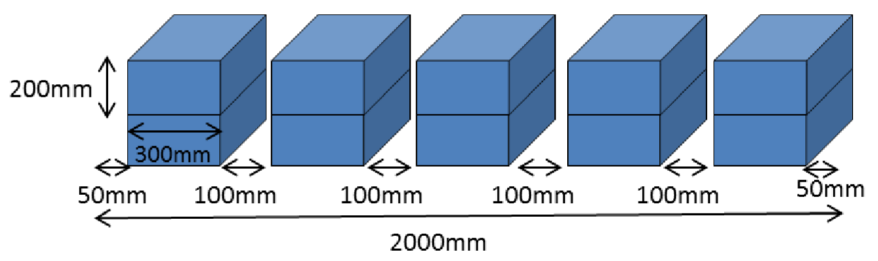
\includegraphics[width=100mm]{Image/ブロック.png}
				\caption{競技中の箱配置}
				\label{ブロック}
			\end{center}
		\end{figure}

		\begin{figure}[htp]
			\begin{center}
				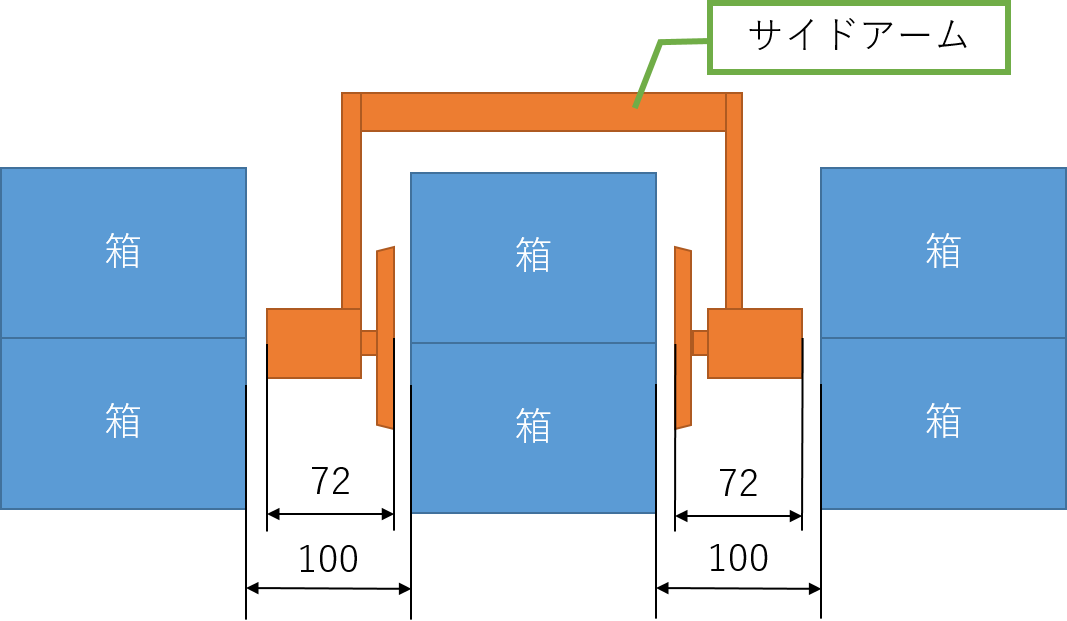
\includegraphics[width=80mm]{Image/箱回収位置寸法.png}
				\caption{箱の幅とアームの幅}
				\label{箱回収位置寸法}
			\end{center}
		\end{figure}

		\begin{figure}[htp]
			\begin{center}
				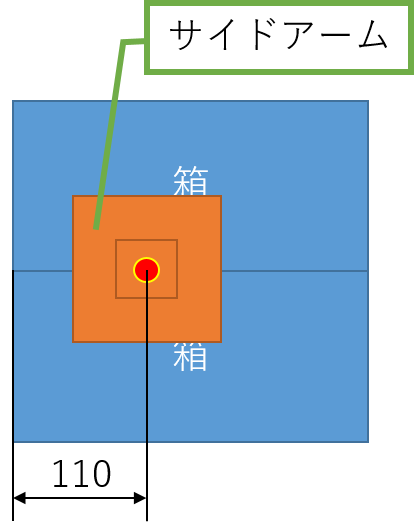
\includegraphics[width=60mm]{Image/箱回収(側面).png}
				\caption{箱回収側面位置}
				\label{箱回収側面位置}
			\end{center}
		\end{figure}

		\subsection{塔建て}
		運んだ箱を高さ750mmの台の上に持ち上げて、下段が大きく上段が小さくピラミッド型のように組み立てる。これは「高台」と「丘」によって異なり、「高台」では図\ref{高台の箱積}のように2列1列1列の順に組み立てる。「丘」では図\ref{丘の箱積}のように下段が上段よりも両側25mm程大きければいくらでも積んで良いとなっている。
		製作した積み込みロボットは「丘」であれば動かずに積み上げることができる。だが「高台」の場合は1列に2段積み上げる必要があるため真横に並行移動できると時間短縮になる。

		\begin{figure}[htp]
			\begin{center}
				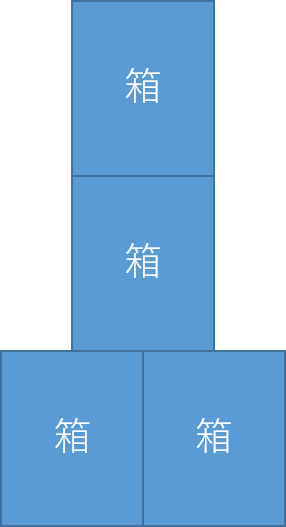
\includegraphics[width=30mm]{Image/高台箱積.png}
				\caption{高台の箱積}
				\label{高台の箱積}
			\end{center}
		\end{figure}

		\begin{figure}[htp]
			\begin{center}
				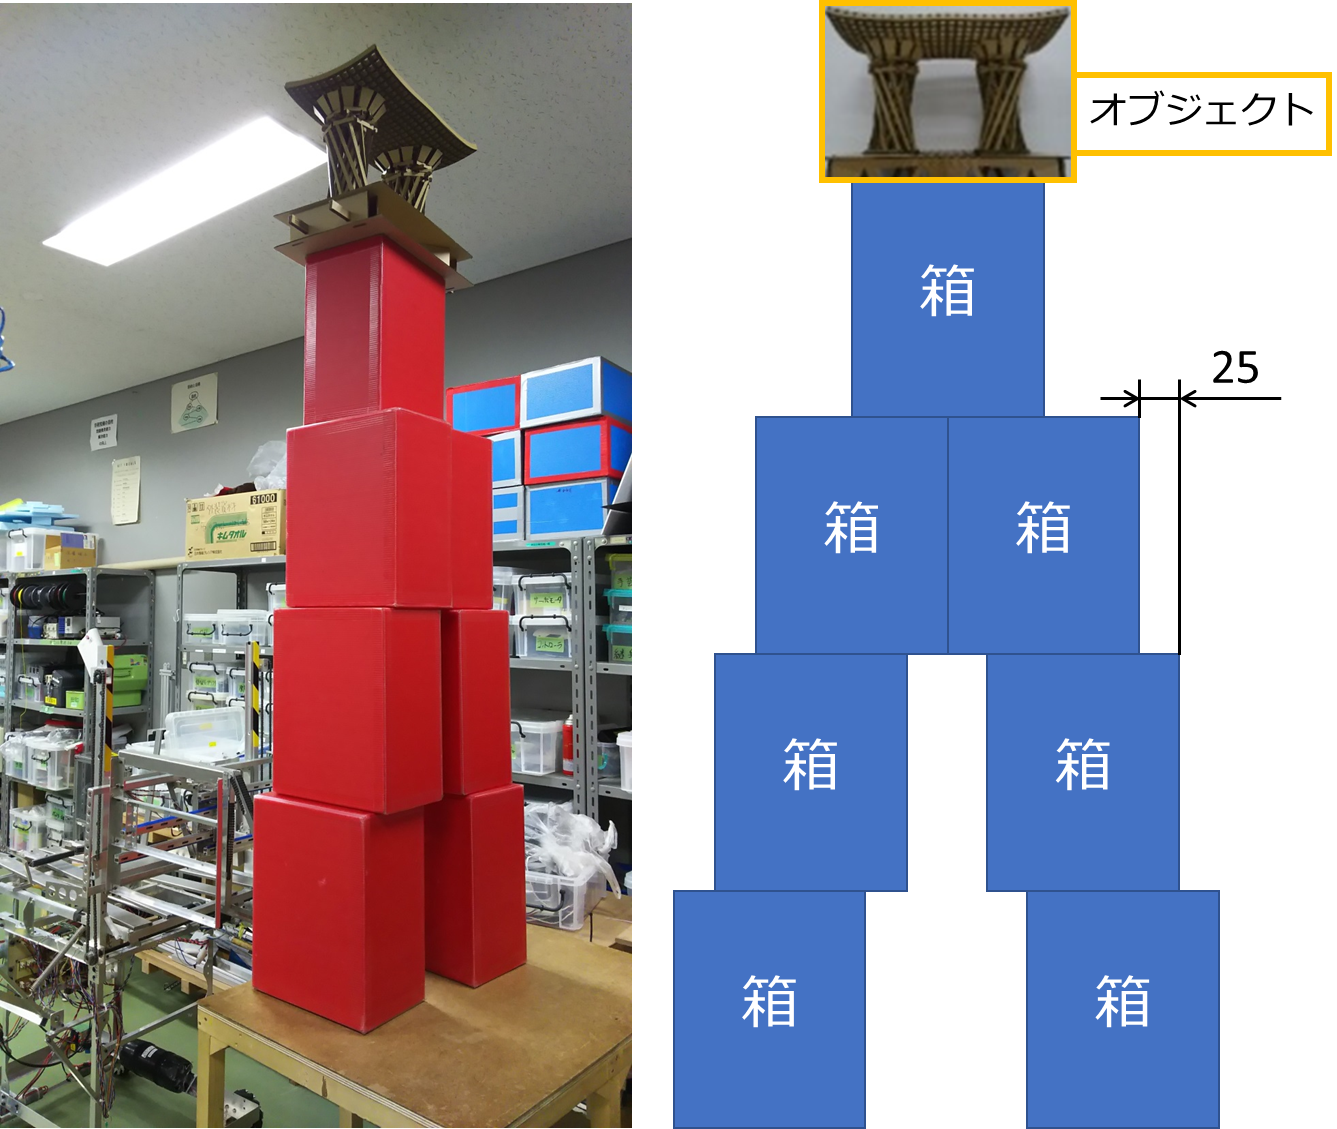
\includegraphics[width=90mm]{Image/丘の箱積.png}
				\caption{丘の箱積}
				\label{丘の箱積}
			\end{center}
		\end{figure}

		\subsection{橋渡り}
		架橋ロボが設置した橋の上を渡るが、その橋に侵入する際に橋幅約80mmでタイヤ2輪同時侵入の位置調整は難しく、2輪駆動だと時間が掛かる。そのため、並行移動できるメカナムホイールは2輪駆動よりスムーズに位置調整が可能である。

		\subsection{オブジェクトの持ち運び}
		丘の左または右に設置されているオブジェクト置き場からオブジェクトの鼓門を持ち運び砦のてっぺんに設置する、この際2輪駆動では旋回を何度も必要となるため、並行移動ができるメカナムホイールが有効的である。

\chapter{メカナムホイールの説明}

	\section{メカナムホイールについて}
	メカナムホイールとは車輪の円周面に回転軸から図\ref{角度}のように45度傾いた樽状のタイヤを一定の間隔を空けながら覆うようにして取り付けた外見をしている。これは車と同じように左右で2輪ずつの計4輪で運用する。メカナムホイール一輪につきモータ一個を取り付け、各モータごとに任意の回転制御を与えることで任意の方向に移動することができる。

	\begin{figure}[htp]
		\begin{center}
			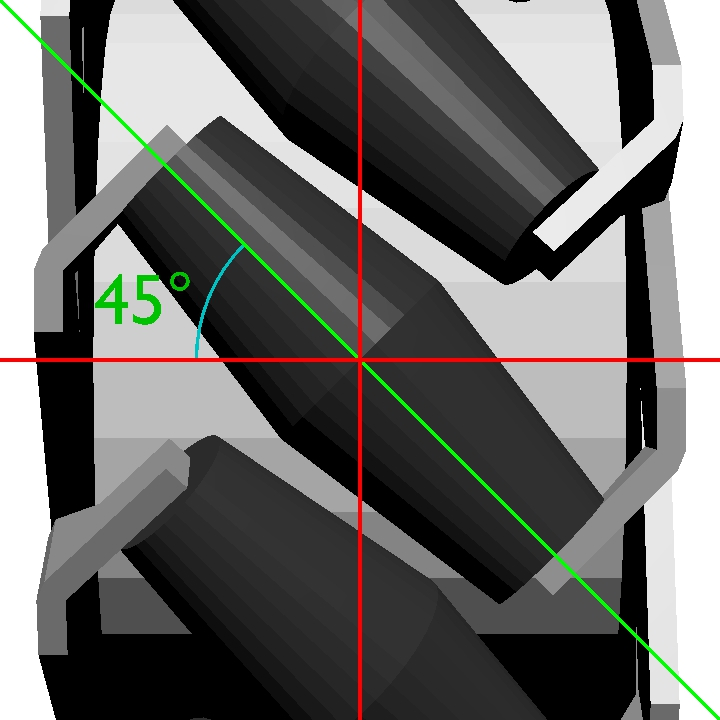
\includegraphics[width=60mm]{Image/角度.jpg}
			\caption{タイヤの角度}
			\label{角度}
		\end{center}
	\end{figure}

	\section{ホイールの向きと組み合わせ}
	メカナムホイールには順方向に傾いた車輪と逆方向に傾いた車輪の二種類があり、図\ref{角度}を順方向とする。これらを左右で2輪ずつの計4輪を図\ref{対角}のように取り付けることで正常に動作する。

	\begin{figure}[htp]
		\begin{center}
			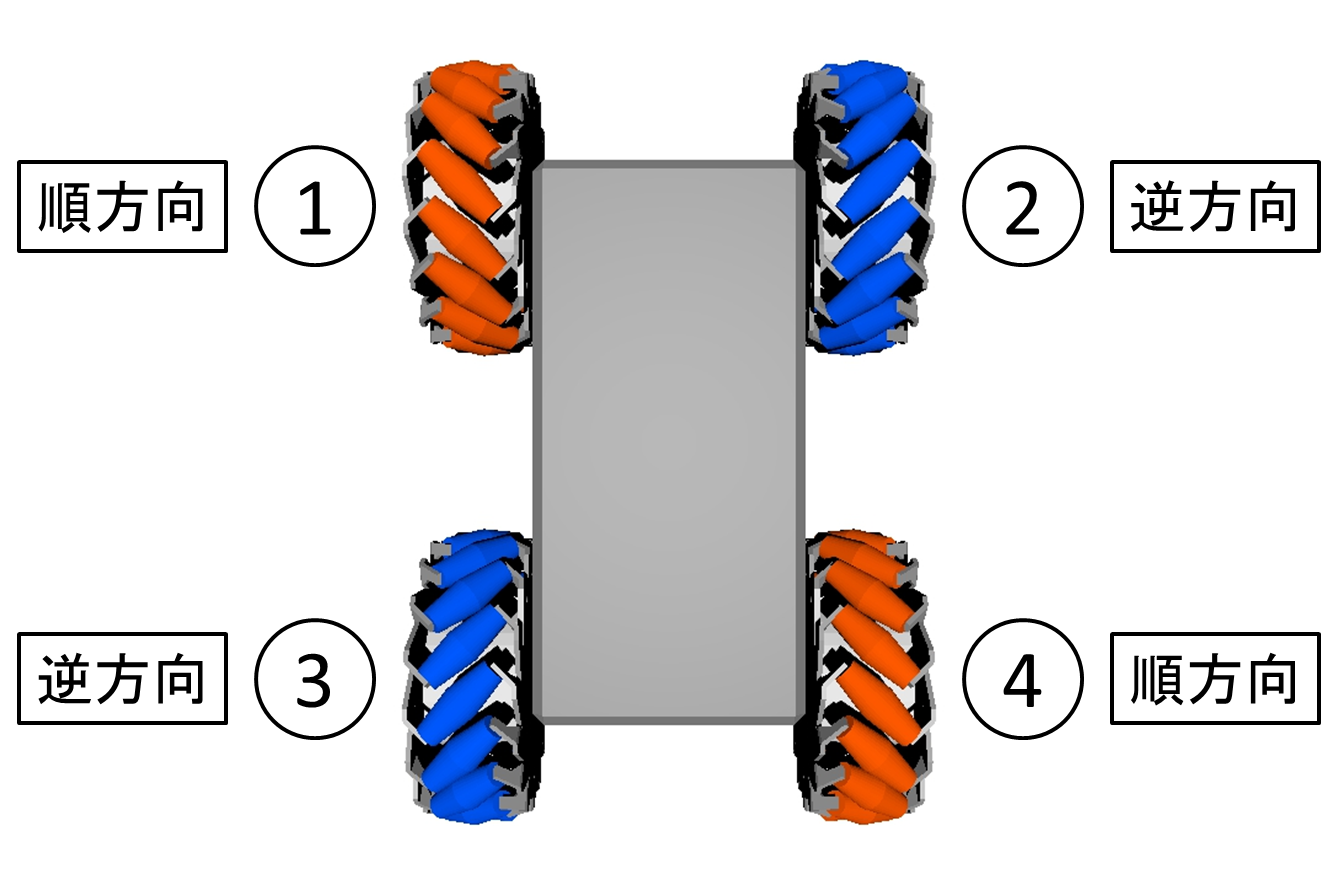
\includegraphics[width=80mm]{Image/対角.png}
			\caption{組み合わせ}
			\label{対角}
		\end{center}
	\end{figure}

	\section{各動作}
	ここではホイール単体の動作と四輪を組み合わせた全体の動作を説明する。

		\subsection{単体の動作}
		静止した状態では地面に接触しているタイヤの回転方向に進むが、回転時ではその逆方向に移動する。図\ref{回転系}は地面から見たそれぞれの車輪の動きを示している。

		\begin{figure}[htb]
			\begin{center}
				\begin{tabular}{c}
					\begin{minipage}{0.5\hsize}
						\begin{center}
							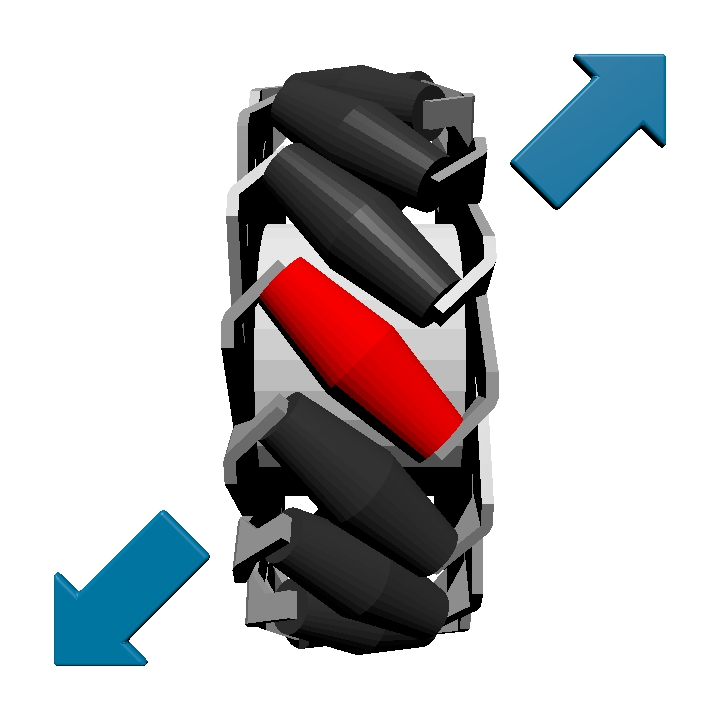
\includegraphics[width=60mm]{Image/無回転.jpg}
							\\(a)無回転
						\end{center}
					\end{minipage}
					\begin{minipage}{0.5\hsize}
						\begin{center}
							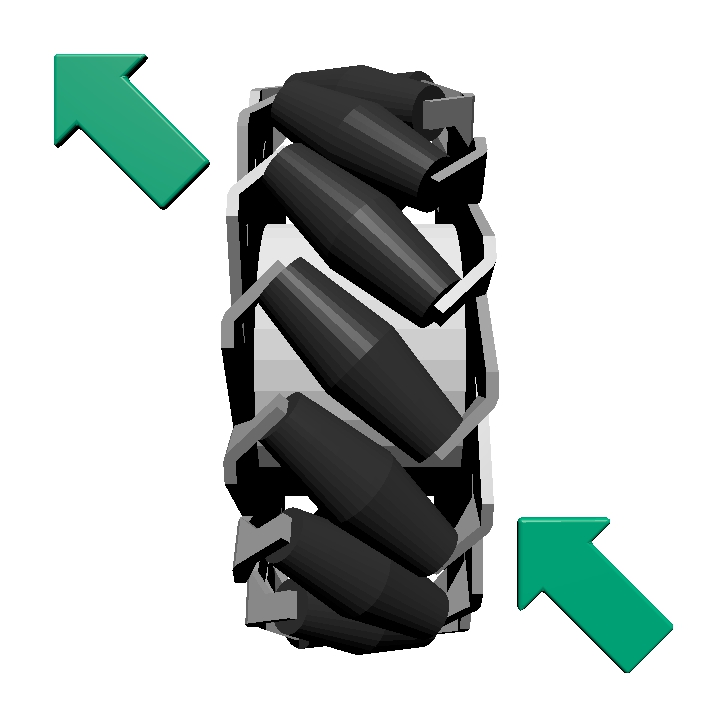
\includegraphics[width=60mm]{Image/回転.jpg}
							\\(b)回転
						\end{center}
					\end{minipage}
				\end{tabular}
				\caption{地面から見た車輪の動き}
				\label{回転系}
			\end{center}
		\end{figure}

		\subsection{全体の動作}
		四輪の状態での動作は車輪の回転によって発生するX方向もしくはY方向のベクトルを互いに打ち消し合うことで、図\ref{移動系}に示すように任意の方向に並行移動することができる。

		\begin{figure}[htb]
			\begin{center}
				\begin{tabular}{c}
					\begin{minipage}{0.33\hsize}
						\begin{center}
							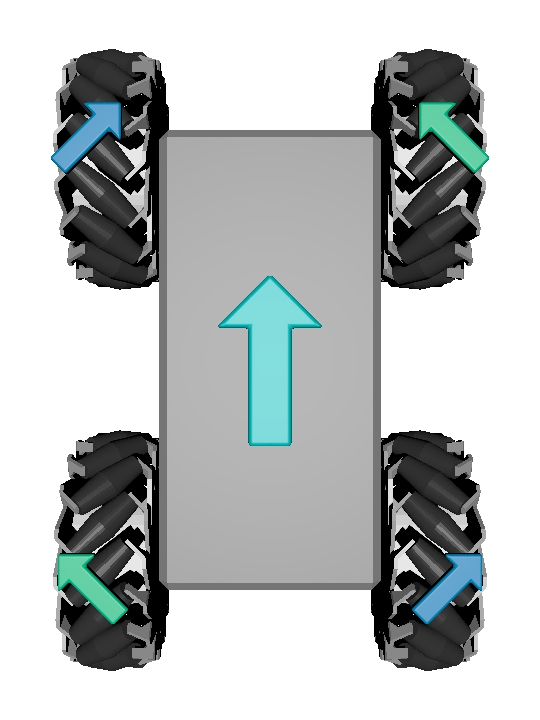
\includegraphics[width=40mm]{Image/ロボット1}
							\\(a)前進
						\end{center}
						\begin{center}
							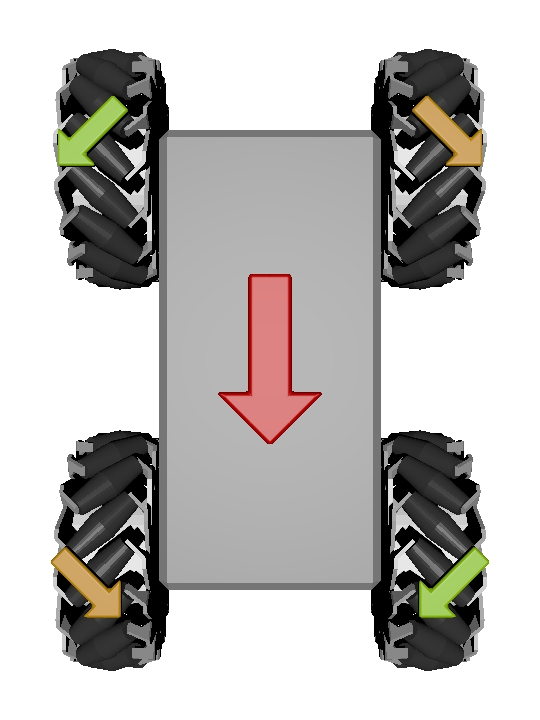
\includegraphics[width=40mm]{Image/ロボット2}
							\\(b)後進
						\end{center}
					\end{minipage}
					\begin{minipage}{0.33\hsize}
						\begin{center}
							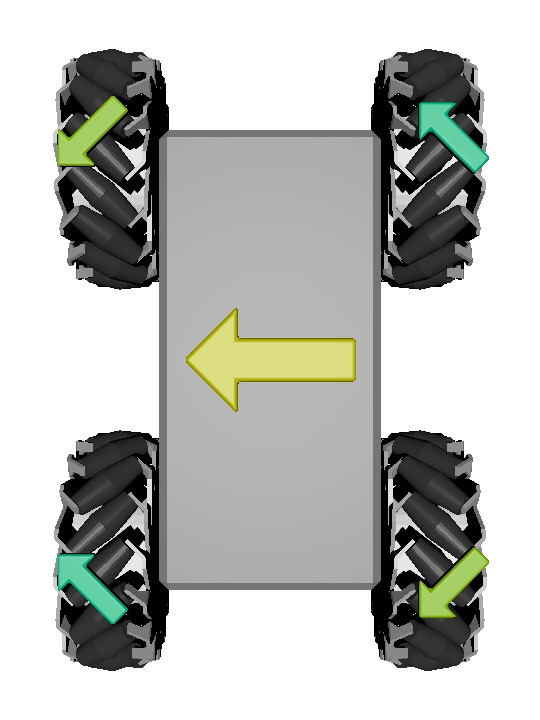
\includegraphics[width=40mm]{Image/ロボット3}
							\\(c)左並進
						\end{center}
						\begin{center}
							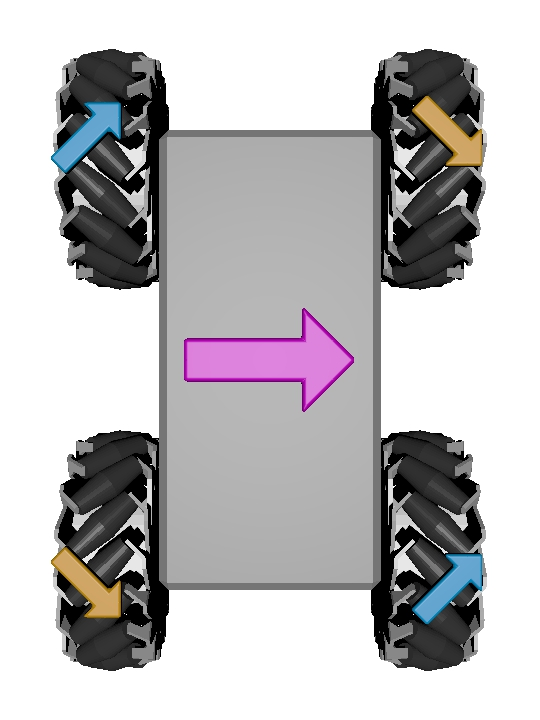
\includegraphics[width=40mm]{Image/ロボット4}
							\\(d)右並進
						\end{center}
					\end{minipage}
					\begin{minipage}{0.33\hsize}
						\begin{center}
							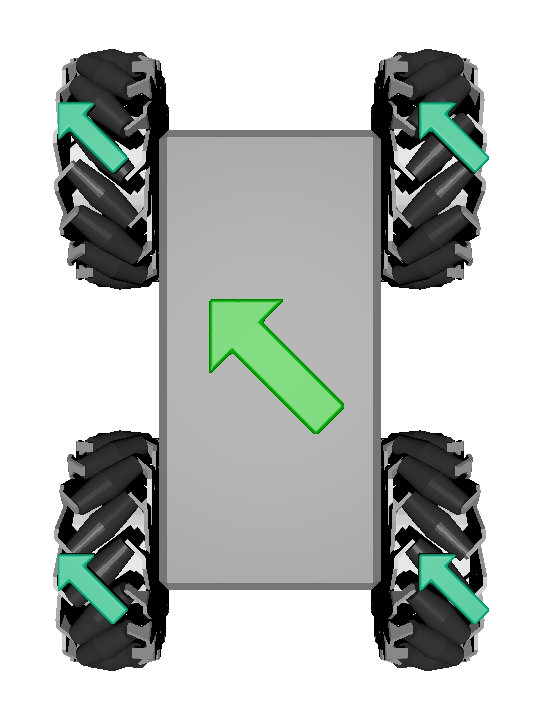
\includegraphics[width=40mm]{Image/ロボット5}
							\\(e)左斜め移動
						\end{center}
						\begin{center}
							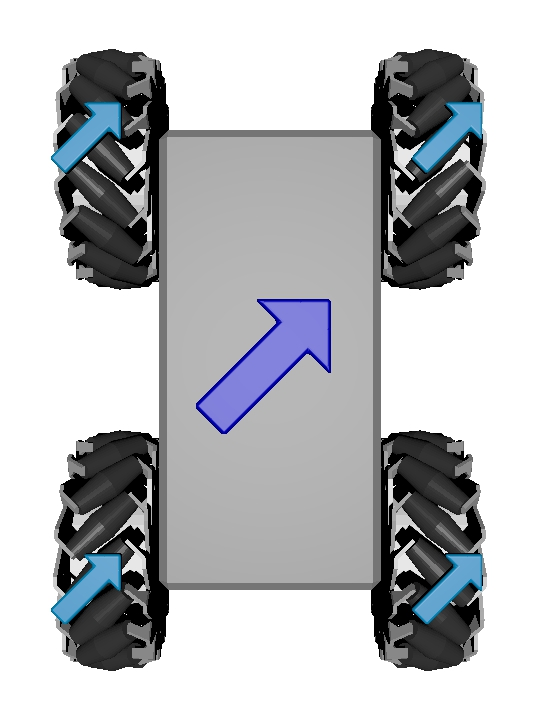
\includegraphics[width=40mm]{Image/ロボット6}
							\\(f)右斜め移動
						\end{center}
					\end{minipage}
				\end{tabular}
				\caption{車輪のベクトルと本体の進行方向}
				\label{ロボット}
			\end{center}
		\end{figure}

	\section{操作プログラム}
	ここではメカナムホイールの回転数を制御する計算式や、そのために必要な定義などを説明する。

		\subsection{定義}
		メカナムホイールを操作するためには縦方向、横方向、回転方向の3種類の値が必要である。さらにこれらを計算してPWM値とするためアナログ値を出力できるコントローラでなければならない。そのため、これらの基準を満たしているDualShock3のアナログスティックを2つ用いて操作する。アナログスティックの初期位置を原点とし、そこからX方向とY方向に傾けることで、その量に応じた値が出力される。左スティックは移動用で倒した方向に並行移動することができる。右スティックは旋回用でこちらはX軸の値しか出力しない。

		\begin{figure}[htp]
			\begin{center}
				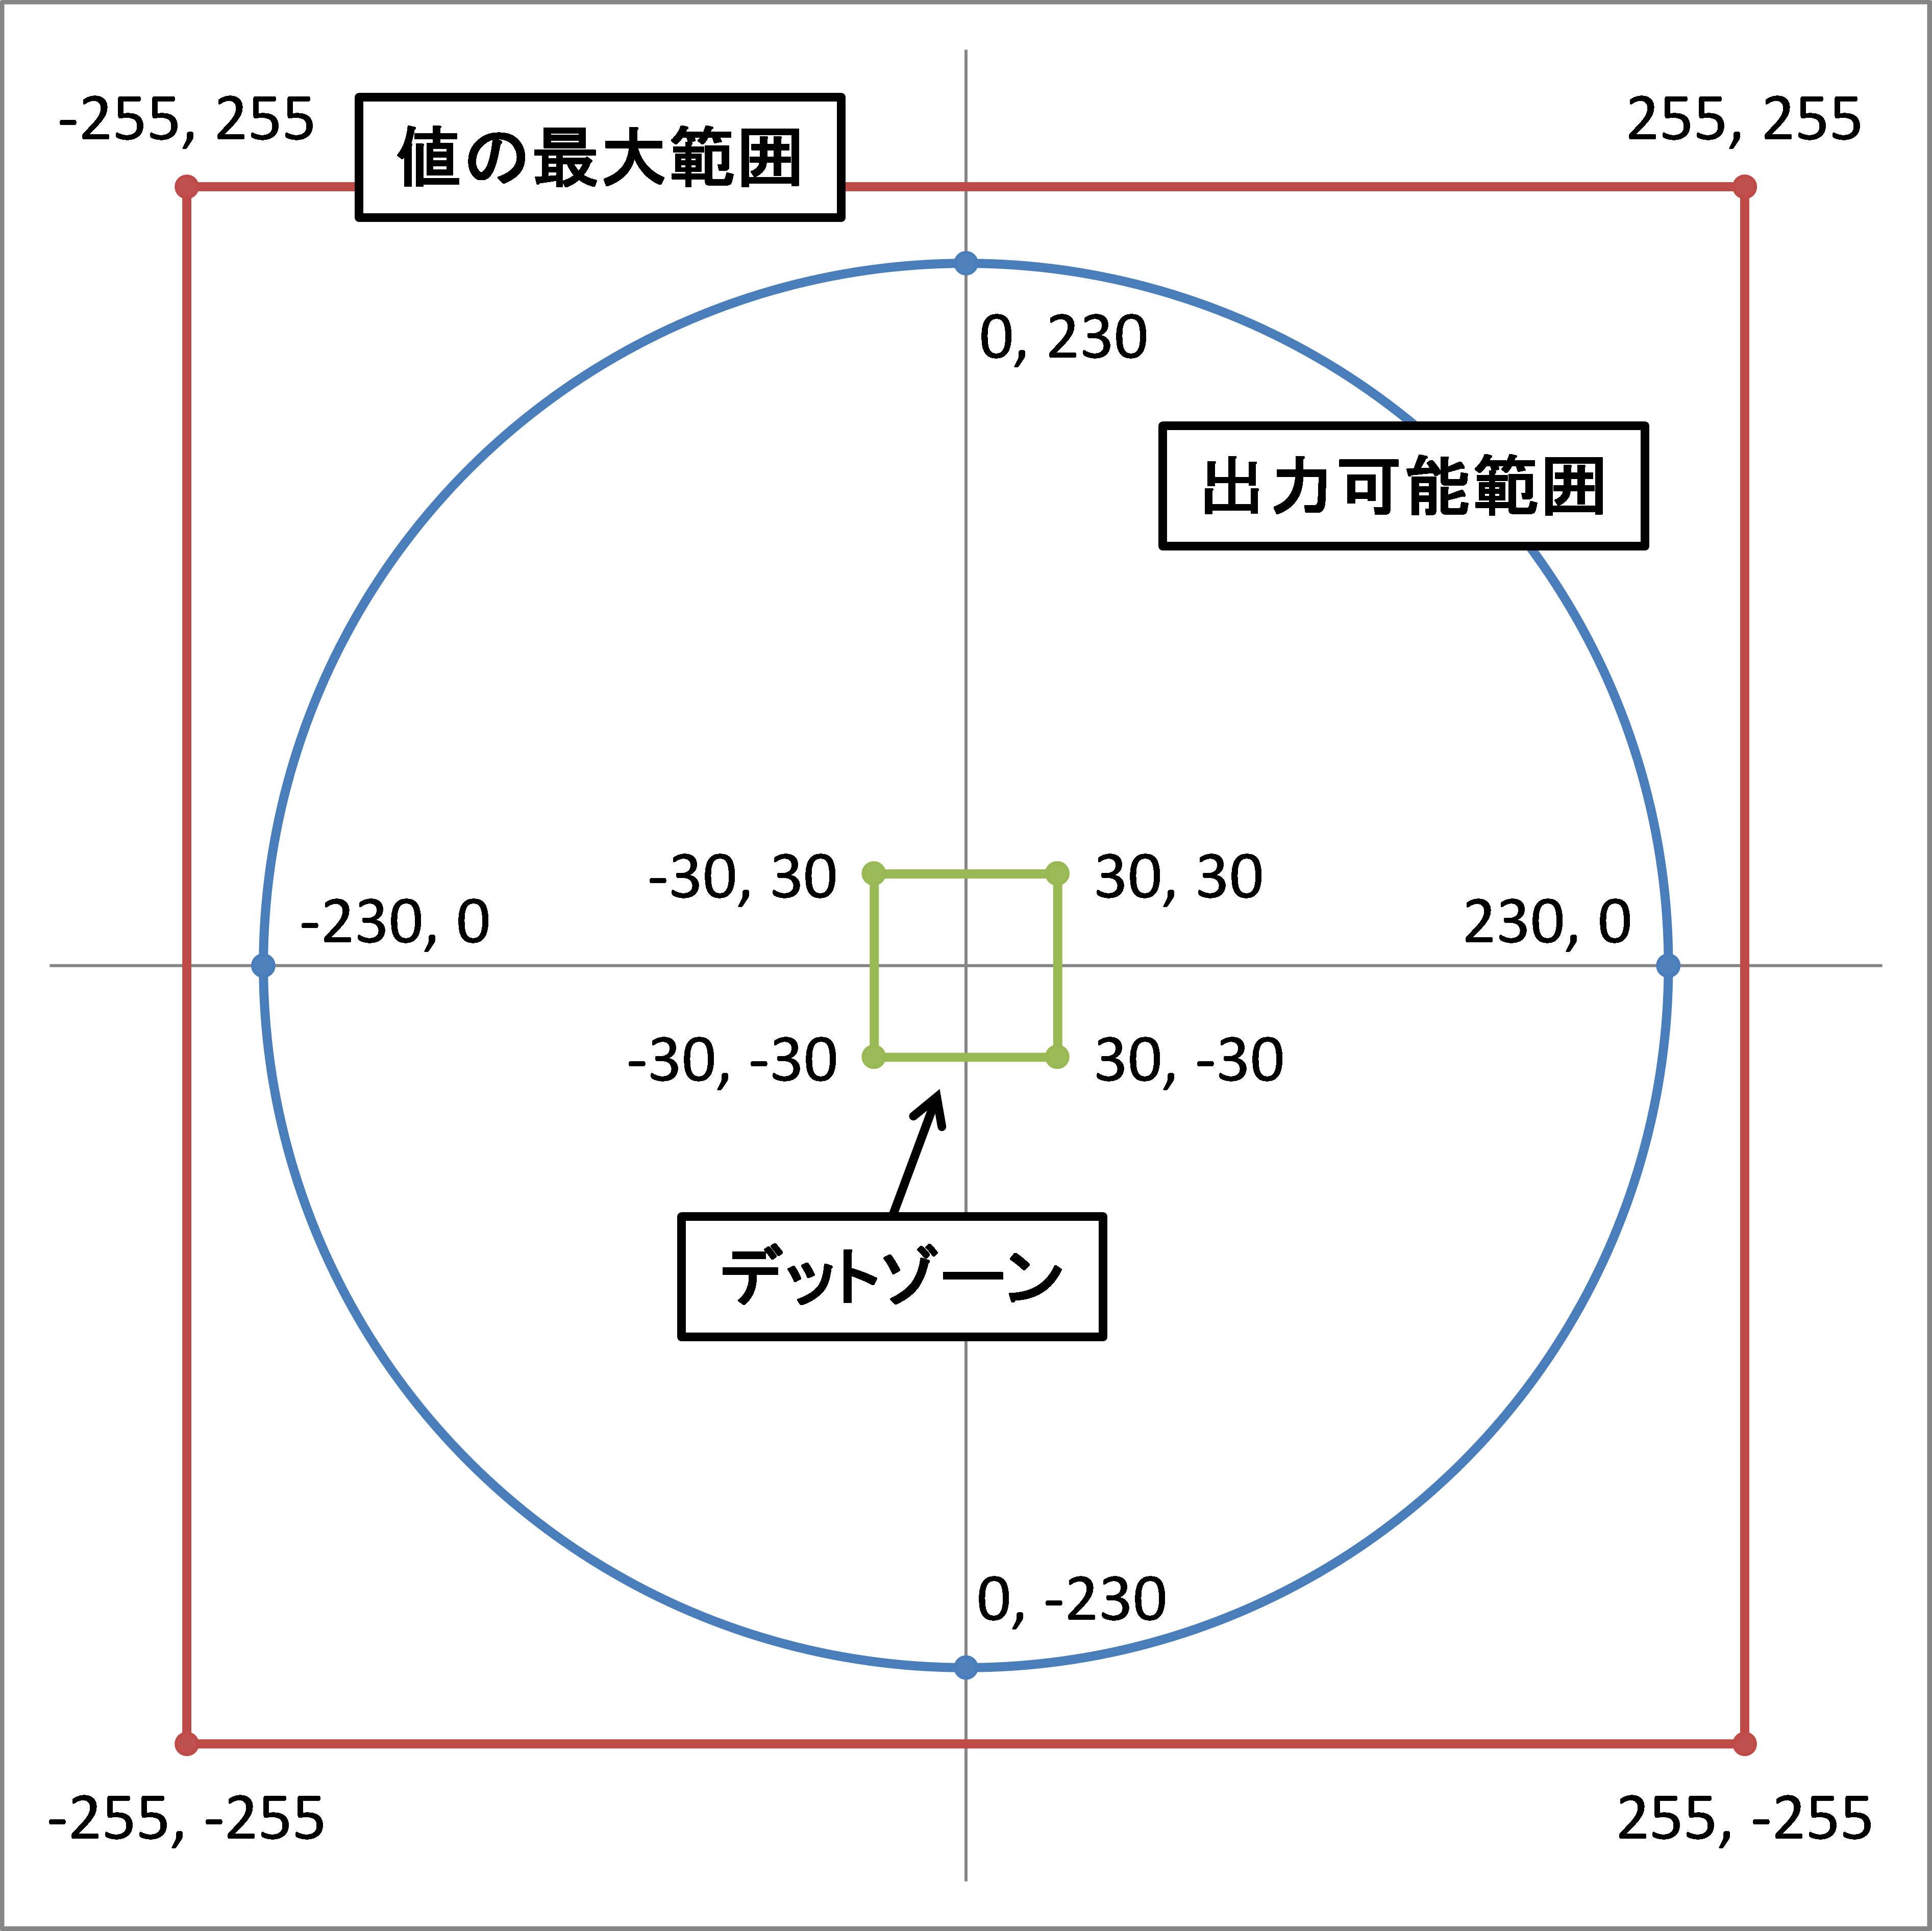
\includegraphics[width=80mm]{Image/座標.png}
				\caption{アナログスティックの座標}
				\label{座標}
			\end{center}
		\end{figure}

		\subsection{計算式}
		左スティックはY方向に傾けることで$L_y$、X方向に傾けることで$L_x$を出力する。右スティックはX方向に傾けることで$R_x$を出力する。モータのPWM値の計算式は以下のようになる。

		\begin{eqnarray}
		M_1 = L_y + L_x + R_x
		\label{式1}
		\\
		M_2 = L_y - L_x + R_x
		\label{式2}
		\\
		M_3 = L_y - L_x + R_x
		\label{式3}
		\\
		M_4 = L_y + L_x + R_x
		\label{式4}
		\end{eqnarray}

\chapter{今回製作したロボットのメカナムホイールの問題点}

	\section{問題点}

	\begin{itemize}
		\item 直進中の環境によって進行方向がずれてしまい斜めに進んでしまう。
		\item 駆動開始時に右方向に大きくずれることがある。
		\item 停止時に慣性で右方向にずれる。
	\end{itemize}
	\label{問題点}

	\section{原因}

		\subsection{項目}
		以下に\ref{問題点}の問題点が発生すると思われる原因を示す。

		\begin{enumerate}
			\item ロボットの重心
			\item 加工精度(タイヤの設置位置)
			\item モータ個々の差
			\item モータドライバの差
		\end{enumerate}

		\subsection{一番の原因と理由}
		この中で一番の原因となっているのは「ロボットの重心問題」である。理由は、図\ref{積み込みロボット重心}に示すように積み込みロボットには、正面に箱を積み上げるためのラックハンド、片方の側面に箱を回収するためのサイドアームが取り付いているため、図\ref{積み込みロボット重心}に示すように重心の位置が中心よりも右上にずれている。これにより左後ろのタイヤが浮くことがあり、4輪全体が均等に床に力を伝えきれないことが問題なのである。

		\begin{figure}[htp]
			\begin{center}
				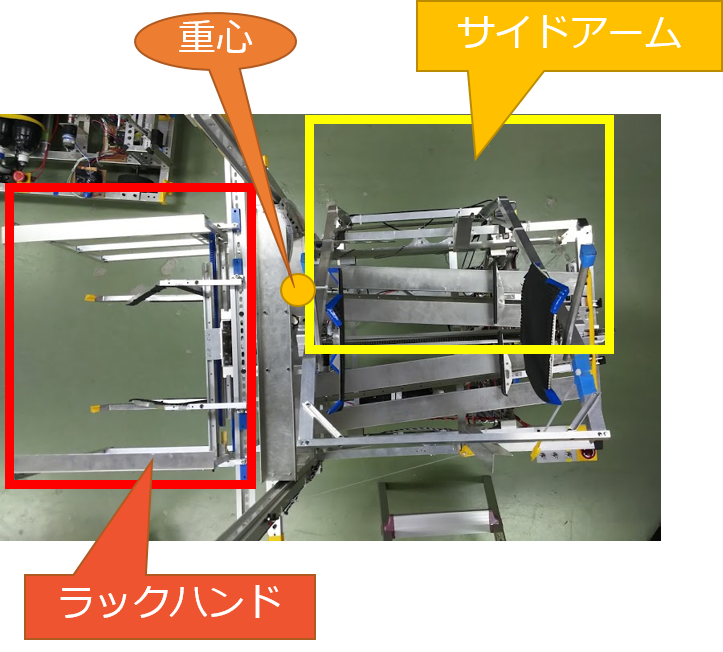
\includegraphics[width=100mm]{Image/積込ロボット重心.png}
				\caption{積み込みロボット重心}
				\label{積込ロボット重心}
			\end{center}
		\end{figure} 

		\subsection{改善無しの直進実験}
		(失敗の例を表として示す予定)
		\label{改善無しの直進実験}

	\section{方向自動修正}
	ロボットの重心が問題であるのならばカウンターウェイトを用いて重心を整えればいいのではないのかと考えられる。しかし、今回のロボコンの競技上、重量制限があるため制御面で改善することにした。そこで用いたのが図\ref{Arduino9軸モーションシールド図}のArduino 9軸モーションシールドでその中に搭載されているジャイロセンサを使用し改善を行った。

\begin{figure}[htp]
		\begin{center}
			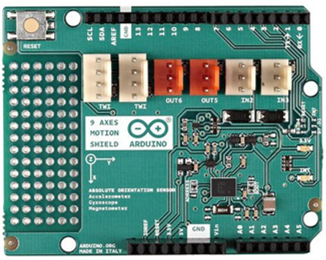
\includegraphics[width=40mm]{Image/Arduino9軸モーションシールド図.png}
			\caption{Arduino9軸モーションシールド図}
			\label{Arduino9軸モーションシールド図}
		\end{center}
\end{figure}

		\subsection{ジャイロセンサ}
		ジャイロセンサとは、角速度センサとも呼ばれ、角度が単位時間当たりにどれだけ変化しているのか計測できるセンサである。このセンサは身近にも用いられており、スマートフォンの加速度センサとの違い、加速度センサは重力方向によって左右上下の認識を行う。

		\subsection{どのような動きか(式に入れることも)}
		今回使用したプログラムでは$-180~180[deg]$の角度を読み取ることが可能で$0[deg]$からずれた分を補正値のPWM値として式\ref{式1},\ref{式2},\ref{式3},\ref{式4}にerrの形で代入し以下のような式となる。

\begin{eqnarray}
M_1 = L_y + L_x + R_x + err
\\
M_2 = L_y - L_x + R_x + err
\\
M_3 = L_y - L_x + R_x + err
\\
M_4 = L_y + L_x + R_x + err
\end{eqnarray}

このようにすることでDualshock3の左スティックを入力中も旋回の動作が自動で行われて自動方向修正が可能となる。

		\subsection{結果}
		(\ref{改善無しの直進実験}の直進実験からどのような変化があったか)

%%%%%%%%%%%%%%%%%%%%%%%%%%%%%%%%%%%%%%%%%%%%%%%%%%%%%%%%%%%%%%%%
\chapter{おわりに}
メカナムホイールを用いることで容易にかつ素早く移動することができるが、ロボットの重心が中心から離れている場合、正しく移動することができない。それを改善するためには原因を修正するか、ジャイロセンサなどで補正する必要がある。

% 参考文献
\begin{thebibliography}{1}
\bibitem{gyro} Arduino9AxesMotionLibrary,http:{\slash}{\slash}www.arduino.org{\slash}learning{\slash}reference{\slash}9-axes-motion,2017{\slash}01{\slash}16閲覧
\end{thebibliography}

\chapter*{謝辞}

\addcontentsline{toc}{chapter}{謝辞}

%%%%%%%%%%%%%%%%%%%%%%%%%%%%%%%%%%%%%%%%%%%%%%%%%%%%%%%%%%%%%%%%
\end{document}

